\chapter{ISPs as adversaries}\label{sec:attack_isp}

Of great importance to our approach, is aquiring real-time network traffic,
with downstream throughput being our only focus; here we discuss the potential
scenarios that allow adversaries to obtain such information, and describe how,
in particular ISPs, could make use of it, to identify video streaming and
profile users based on their streaming habits.

\section{Attack Scenarios}\label{attack_scenarios}

Given the nature of modern Internet infrastructure, an adversary interested in
eavesdropping a particular communication, only needs to compromise a node on
the path the communication travels through. An \emph{on-path} attacker could
easily gain passive access to network and transport layers, and start capturing
network traffic. This can include malicious or compromised Wi-Fi access
points, routers, tapped network cables and ISPs. 

Rather than just attacking physical devices, leaks of information could occur
in network connections, in which an attacker physically close to the victim,
could make use of a \emph{Wi-Fi sniffer} to estimate traffic by capturing
physical layer WLAN packets.  Information may be encrypted by 802.11, and the
sniffer may not take into account packet retransmissions at the session layer
nor multiple TCP/IP flows on the same link, potentially causing noise on the
observation. Despite so, Reed et Al. \cite{leaky_streams}, have shown that it
is still possible to estimate WAP-to-client throughput and use it to identify
the content being streamed.

In addition to the above, \emph{side-channel eavesdropping} can exploit
information about the network structure, to saturate a link between the user
and the server, and estimate fluctuations of congestion by sending probes
remotely and observing queueing delays in routers \cite{side_channel}. 

We will now present the relevant phases and tools needed for an ISP to perform
an attack, considering the ISP an \emph{on-path} attacker.

\section{Video Fingerprinting}

Assuming that the ISP has no direct access to the CDN titles are stored in, it
needs to build a database of video traffic to match against future video stream
captures. To build such a database, the ISP needs to have access to a network
interface, control its inbound bandwidth, (to get different levels of quality
for each title), and capture incoming traffic passing through it.

In order to control the incoming bandwidth, the ISP could either limit it
directly onto a generic L4 switch, or decide to connect
any UNIX-like machine and throttle the throughput of its main ethernet
interface. We will consider the scenario in which the ISP limits the bandwidth
of the ethernet interface of the switch, (less noisy and more stable).

The value of the enforced bandwidth determines the quality (bitrate) of the
content that will be captured. Assuming that each title has a unique bitrate
ladder, the ISP should come up with an ad-hoc policy for every video to
faithfully reconstruct the quality levels of it. While correct, a more viable
approach to this problem, would be to just consider a range of bitrates capable
of spanning the space of possible quality levels. 

In our own version of the attack, presented in \Cref{sec:approach}, we use
the values in \Cref{tab:bandwidths}. 

\begin{table}[htb]
  \centering
  \begin{tabular}{|c|c|c|c|c|c|c|c|c|c|c|c|c|}
    \hline
    \multicolumn{13}{|c|}{\textbf{Bandwidth levels (Mbps)}} \\
    \hline
    0.6 & 0.8 & 1.2 & 2 & 3.5 & 4.2 & 4.8 & 5.5 & 6.5 & 7.05 & 10 & 15 & 20 \\ 
    \hline
  \end{tabular}
  \caption{Enforced bandwidth levels.}
  \label{tab:bandwidths}
\end{table}

The ISP can now connect a UNIX-like machine to the switch's network interface
with bandwidth limit \emph{b}, and invoke \texttt{adudump} to infer the size of
each \emph{application data unit} ADU by processing TCP/IP packet header
traces that generate \emph{a-b-t} connection vectors \cite{hernandez}.

\subsection{The a-b-t model}

The lifetime of a TCP endpoint that sends and receive data units is not only
dictated by the time spent on these operations, but also by quiet times in
which the TCP connection remains idle, waiting for upper layers to formulate
new demands. Clearly, longer lifetimes may have a huge impact overall, due to
the fact that resources needed to handle TCP state, remain reserved for a
longer time. In contrast, ADUs that are sent within a short period of time, get
aggregated by the TCP window mechanism, reducing the exchange of
requests/responses between source and destination.

These ideas have been formalized into the \emph{a-b-t model}, that describes
TCP connections as sets of ADU exchanges and quiet times. The term a-b-t is
descriptive of the building blocks of the model: \emph{a-type} ADUs, sent from
the connection initiator to the connection acceptor, \emph{b-type} ADUs, sent
from the responder back to the initiator, and quiet times \emph{t}'s, during
which, no data segments are exchanged.

The model has two different flavors depending on whether ADU interleaving is
sequential or concurrent: the former is used for modeling connections for which
only one ADU is sent from one endpoint to the other at a given point in time,
(one endpoint will wait until the other has completed the transmission of the
current ADU before sending a new one), while the latter is used for modeling
connections in which both endpoints send and receive ADUs simultaneously.

As one can notice from a sample traffic trace from Netflix, the two endpoints
behave in a sequential fashion, as shown by the \texttt{SEQ} flag in
\Cref{lst:adutrace}.

\begin{adu}[caption={Incoming traffic trace of Mulan, captured at 10Mbps (first 10 segments).}, label={lst:adutrace}]
ADU: 1565880580.152388 192.168.0.157.54924 <1 45.57.19.134.443 198837 SEQ 0.804088
ADU: 1565880581.321246 192.168.0.157.54924 <1 45.57.19.134.443 198760 SEQ 0.907568
ADU: 1565880582.688335 192.168.0.157.54924 <1 45.57.19.134.443 199407 SEQ 1.052862
ADU: 1565880591.912352 192.168.0.157.54974 <1 45.57.19.134.443 525046 SEQ 0.058709
ADU: 1565880592.168340 192.168.0.157.54968 <1 45.57.19.134.443 275568 SEQ 0.558654
ADU: 1565880592.168344 192.168.0.157.54974 <1 45.57.19.134.443 305115 SEQ 0.062028
ADU: 1565880592.172495 192.168.0.157.54982 <1 45.57.19.134.443 198735 SEQ 0.670224
ADU: 1565880592.697314 192.168.0.157.54974 <1 45.57.19.134.443 236474 SEQ 0.179115
ADU: 1565880592.820292 192.168.0.157.54982 <1 45.57.19.134.443 286547 SEQ 0.106913
ADU: 1565880592.820395 192.168.0.157.54968 <1 45.57.19.134.443 198530 SEQ 0.310506
\end{adu}

\subsection{Inference}

\begin{figure}[!h]
  \centering
  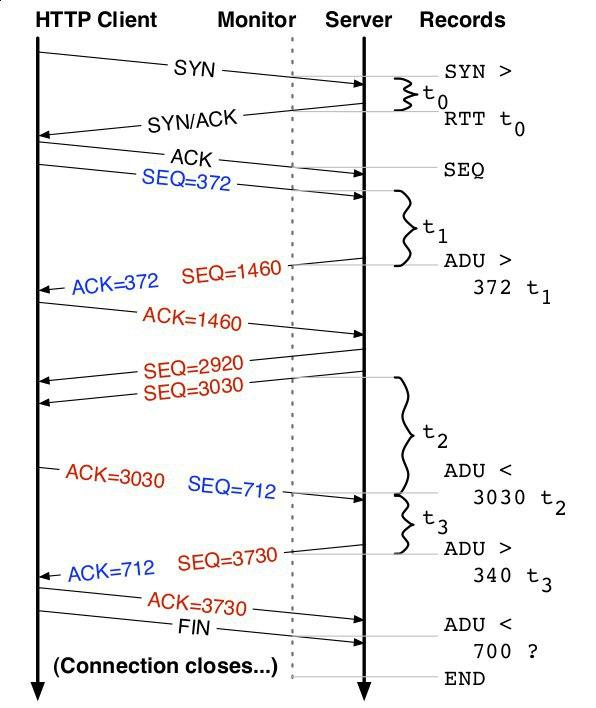
\includegraphics[width=0.6\columnwidth]{img/adudump.png}
  \caption{Detailed segment size inference in adudump.}
  \label{fig:adudump}
\end{figure}

\Cref{fig:adudump} shows an example of how Adudump's inference process works.
The connection starts when the three-way handshake completes, (marked as a
\texttt{SEQ} record). The monitor then records the time the first data segment
is sent from the client. The server then acknowledges the previous request, and
adudump infers the size of the completed ADU to be 372 bytes, generating a
record with the ADU's size direction and think-time. Note how adudump generates
no record until it infers that the ADU is complete, moreover the think times
reported, are relative to the position of the monitor in the network, the
farthest the monitor is from the server, the noisiest the measure of quiet
times becomes. More on the effect of quiet times is described in
\Cref{sec:approach}.

\subsection{Identifying Netflix traffic}

In order to identify specific video traffic from a Netflix CDN, the ISP could
either inspect the DNS response packets or the TLS handshake messages, and
perform a DNS lookup for each video every time, or to maintain an updated list
of IP addresses with mappings to the recorded traffic. Then all the ISP is left
with, is a mixed trace of audio and video segments. Each Netflix audio segments
represents about 16 seconds of playback, while every video segment corresponds
to a 4 second playback. The ISP could now decide to either filter out audio
segments by either thresholding on the size of ADUs, as done by Reed et Al (at
200 kilobytes), or to consider audio as part of the fingerprint of a title. The
200 kilobytes threshold represent a good heuristic when considering traces
recorded at high bandwidth levels, in fact, audio segments sizes are around 198
kilobytes, whereas if considering the same title at a low level of bandwidth
(less than 1 Mbps indicatively), one cannot distinguish audio and video
segments by their size. For this reason, we consider an approach that does not
filter out audio segments. In \Cref{sec:approach} we highlight the difference
between the two methods.

\subsection{Building a database of fingerprints}

The ISP can now automate the streaming of Netflix videos, and build a database
of such fingerprints. Here, the ISP is free to use a method of storage of
choice, depending on the granularity of the features required to represent each
title, and on the cardinality of the set of titles it wants to capture.  In
addition, as Netflix is constantly adding/removing titles from its library, the
ISP is required to constantly keeping updated the database to guarantee that
the attack can target newly added titles.

\newpage

\section{Capturing video traffic}

In order to capture video traffic to match it against a database of collected
fingerprints, it requires the ISP to be in possess of a generic L4 switch
capable of mirroring traffic from a port to another one. Then any UNIX-like
system that implements \emph{libpcap} is suitable for capturing inbound traffic
on the mirrored port, as presented below in \Cref{fig:schema}.

\begin{figure}[!htb]
  \centering
  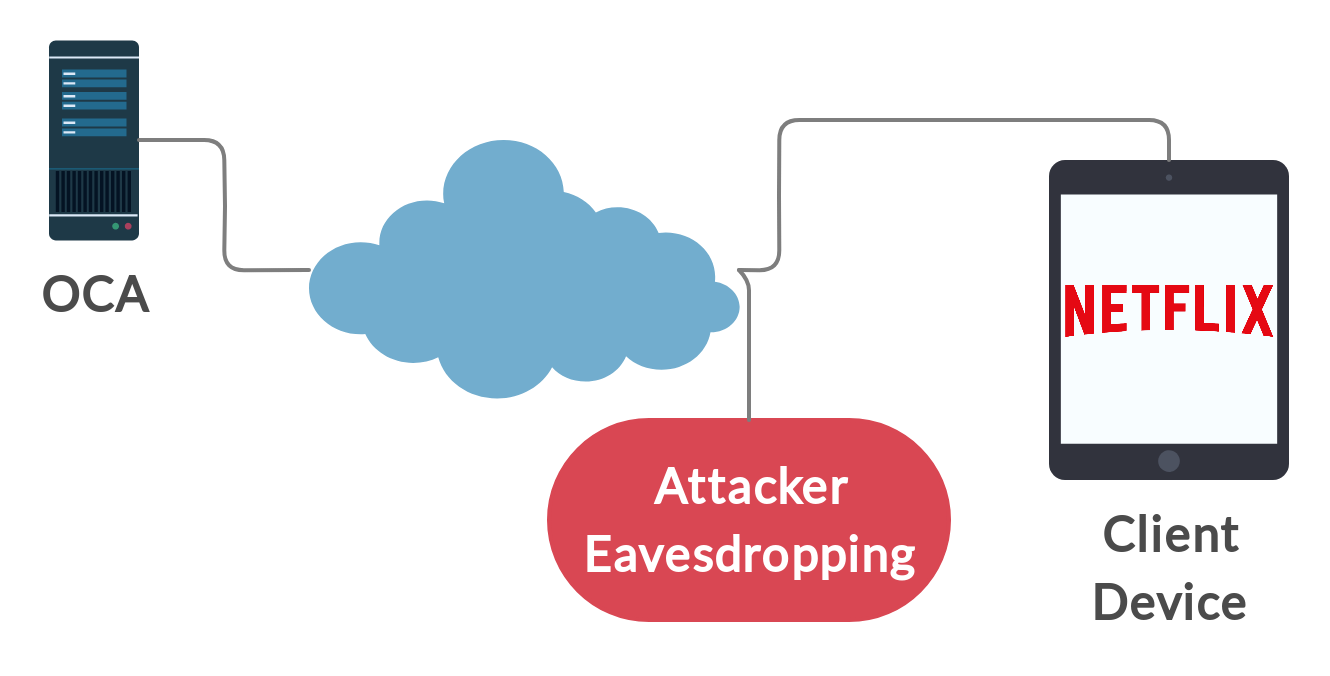
\includegraphics[width=\columnwidth]{img/schema.png}
  \caption{Traffic capture scenario.}
  \label{fig:schema}
\end{figure}

In this scenario, the client is unaware of the fact that its traffic is being
mirrored and recorded by the ISP, and there is no practical way for him to
claim that. On the other hand, a user concerned with its privacy, may avoid
such attack.

\subsection{Possible countermeasures}

In order to safely stream Netflix videos without the ISP being able to identify
the content of them, a user particularly concerned about its privacy, (e.g.
public figures, politicians, government agency employees), may decide to use a
VPN. When using a VPN, the user, still needs the ISP to connect to the
internet, but instead of having the ISP communicating directly with the desired
resource, the ISP now "talks" with the VPN server. It is responsibility of the
VPN server in fact, to establish a communication with the webpage the user
wants to access.  The key point is that the client and the VPN server establish
a secure connection (VPN tunnel). Thus, as long as the user's VPN of choice,
encrypts data transfer, either with IPSec's \textbf{Encapsulated Security
Payload} or, in case of a remote-access VPN, with PPP's based protocols such as
L2F, PPTP or LT2P, the user is guaranteed that its traffic cannot be
intercepted by the ISP. This is feasible as long as both the VPN software
provides an automatic kill switch to avoid dropouts, and the online resource
does not restrict access to user connected via VPN. 

Netflix prevents the use of VPN
software to prevent users to access to other countries catalogue, although
certain VPN clients are able to bypass this check \cite{nordvpn}.
